\lab{Correlation and Covariance}{Correlation and Covariance}
\label{lab:Stats1}

\objective{Explore applications of inner product spaces to topics in statistics.}

% Source of the datasets: http://people.sc.fsu.edu/~jburkardt/datasets/regression/regression.html
% under the GNU LGPL liscence

\section*{Shifting Data by the Mean}
When analyzing numerical data, it is often useful to transform the data to have an average value of 0.
This process, which we call shifting by the mean, 
is easily accomplished by simply subtracting the mean of the data from each value. 
The resulting shifted data now shows how each data point deviates from the mean.
This form makes it easier to spot outliers, judge the spread of the data, and compare with other data sets.

Consider Table \ref{tab:data} representing students scores in a class.\\

\begin{figure}
\begin{center}
\begin{tabular}{|c|r|r|r|r|}
	\hline
Student & Homework & Exam 1  & Exam 2 & Final \\
\hline
S1  & 89 & 91 & 77 & 75 \\
S2  & 67 & 72 & 76 & 66 \\
S3  & 72 & 77 & 69 & 70 \\
S4  & 56 & 60 & 55 & 61 \\
S5  & 92 & 98 & 89 & 86 \\
S6  & 83 & 88 & 90 & 84 \\
S7  & 45 & 60 & 55 & 48 \\
\hline
Average  & 72 & 78 & 73 & 70\\
\hline
\end{tabular}\\
\end{center}
\caption{Homework and exam scores for 7 students in a class.}
\label{tab:data}
\end{figure}

We can shift our data set by subtracting each column by its average value.  
This makes it so that the average of each column is zero.  
If $W$ represents the matrix of scores, the following Python command will shift each column by the mean.
\begin{lstlisting}
>>> W = np.array([[89, 91, 77, 75],
                  [67, 72, 76, 66],
                  [72, 77, 69, 70],
                  [56, 60, 55, 61],
                  [92, 98, 89, 86],
                  [83, 88, 90, 84],
                  [45, 60, 55, 48]])
>>> column_means = W.mean(axis=0)
>>> X = W - column_means
>>> X
array([[ 17.,  13.,   4.,   5.],
       [ -5.,  -6.,   3.,  -4.],
       [  0.,  -1.,  -4.,   0.],
       [-16., -18., -18.,  -9.],
       [ 20.,  20.,  16.,  16.],
       [ 11.,  10.,  17.,  14.],
       [-27., -18., -18., -22.]])
\end{lstlisting}

Once we have subtracted out the mean from a vector, it is a simple task to compute its variance and standard deviation.
The \emph{variance} of an $n$-dimensional vector $v$, often denoted $\sigma^2$, is defined by the formula
\[
\sigma^2 = \frac{1}{n}\displaystyle\sum_{i=1}^n (v_i - \mu)^2,
\]
where $\mu$ is the mean of $v$. The \emph{standard deviation} of $v$ is simply $\sigma$, i.e. the square
root of the variance. These quantities measure the spread of the entries of the vector. When all of the entries are clustered
closely around the mean, the variance is small. See Figure \ref{fig:variance} for an illustration of variance and mean-shifted data.

(Note: \emph{unbiased variance} is a quantity closely related to variance, but defined slightly differently. It comes into play
in particular for small datasets or vectors. Further discussion is beyond the scope of this lab, but be aware that there is
more than one type of variance.)

\begin{figure}
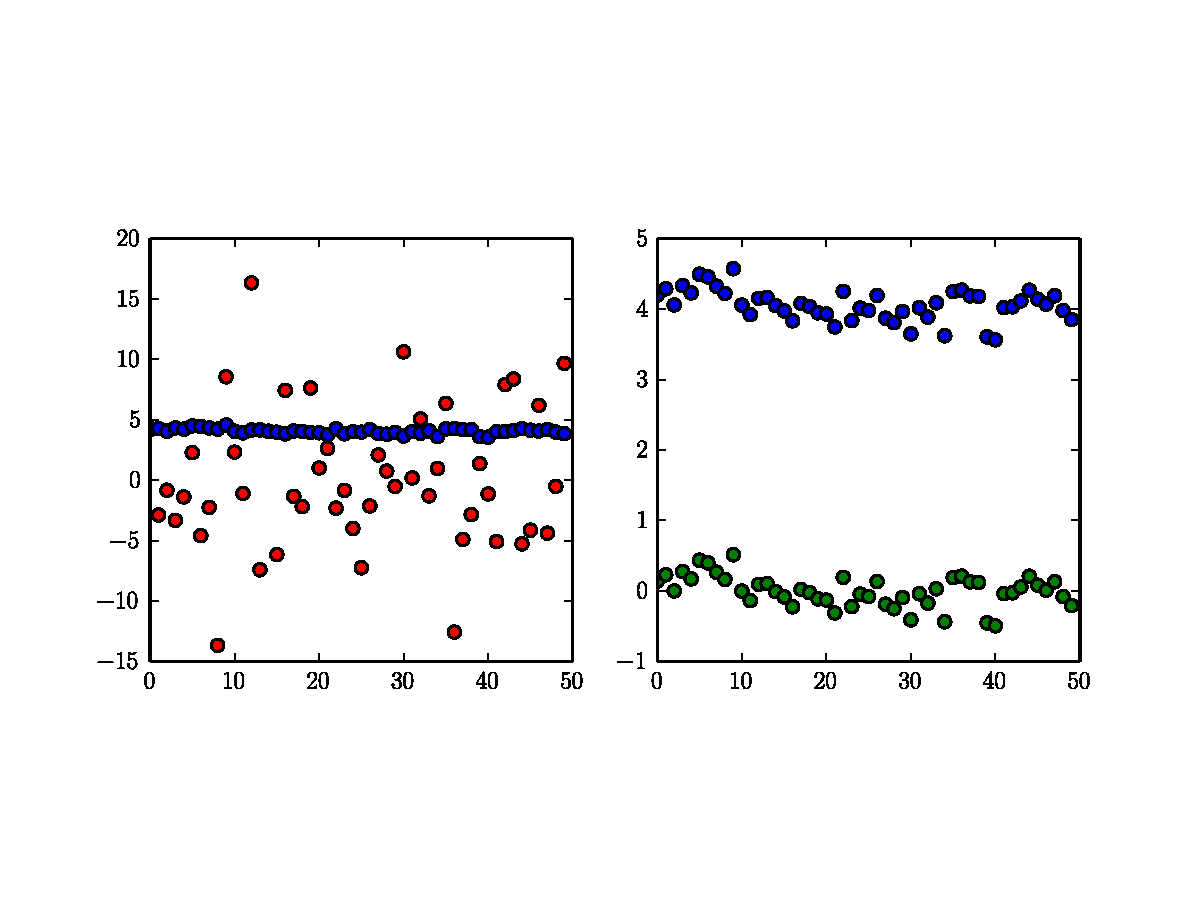
\includegraphics[width=\textwidth]{variance}
\caption{On the left, the red values come from a vector with relatively high variance,
         and the blue values come from a vector with relatively low variance.
         On the right, the green values have been shifted by the mean from the blue values.}
\label{fig:variance}
\end{figure}

Calculating the variance and the standard deviation in Python is straight forward.
Given the shifted data $X$, we simply square each entry, sum along the columns, and divide by the number of rows
to obtain the variance. Take the square root of the result to get the standard deviation.
\begin{lstlisting}
>>> var = (X**2).sum(axis=0)/X.shape[0]
>>> var
array([ 260.     ,  193.42857,  176.28571,  151.14285])
>>> std = np.sqrt(var)
>>> std
array([ 16.124515,  13.907860,  13.277263,  12.294017])
\end{lstlisting}
Observe that the scores for the homework exhibited the largest amount of spread.

As with many things in Python, there is an even shorter, more convenient way to calculate these quantities.
We may calculate the variance and standard deviation of the columns directly from $W$, without having to shift
by the mean.
\begin{lstlisting}
>>> W.var(axis = 0)
array([ 260.     ,  193.42857,  176.28571,  151.14285])
>>> W.std(axis = 0)
array([ 16.124515,  13.907860,  13.277263,  12.294017])
\end{lstlisting}

\begin{problem}
\label{prob:shiftdata}
Import the dataset contained in the \li{weight_age_fat.txt} file. The first row is a header, and contains the names
of each column, but no actual data. There are five columns, but the first two do not contain any data of interest.
The last three columns contain data on the weight (in kilograms), age (in years), and blood fat content of 25
individuals. Distinct data entries are separated by whitespace.

Write a function \li{shiftByMean} that shifts the columns of an input array by their respective means, and returns the result.
Next, write a function \li{computeVariance} that calculates and returns the variance of each column of an input array.
Finally, write a function \li{reportStDev} that accepts no parameters and returns nothing, and simply contains a print
statement that prints out the name of the column with the smallest standard deviation as well as the numerical value of
its standard deviation.

\end{problem}

\section*{The Inner Product and Angles Formula}

Inner products give information about lengths of vectors and angles between vectors.
Recall that the standard inner product on $\mathbb{R}^n$ between vectors $v$ and $u$ is given by
\[
\ipt{v}{u} = v^T u = \displaystyle\sum_{i=1}^n v_iu_i.
\]
We can take advantage of convenient syntax in NumPy to quickly calculate the inner product between two vectors:
\begin{lstlisting}
>>> v = np.array([1., -2., 4.])
>>> u = np.array([2., 3., -1.])
>>> v.dot(u)
-8.0
\end{lstlisting}
The 2-norm of a vector can be easily recovered from the inner product:
\begin{lstlisting}
>>> v_norm = np.sqrt(v.dot(v))
>>> v_norm
4.5825756949558398
\end{lstlisting}
Another option to calculate the norm of an array is to use the \li{numpy.linalg.norm} function, which has the
capability of computing a variety of different types of norms. 
It is also convenient for computing norms of columns or rows of matrices, as follows:
\begin{lstlisting}
>>> from numpy.linalg import norm
>>> # calculate norms of the columns of X
>>> norm(X, axis=0)
array([42.661, 36.797, 35.128, 32.527])
\end{lstlisting}

Recall that the angle $\theta$ between two nonzero
vectors $v$ and $u$ is given by
\[
\cos{\theta} = \frac{\ipt{v}{u}}{\norm{v}\norm{u}}
\]
where $\norm{v} = \sqrt{\ipt{v}{v}}$ denotes the 2-norm of $x$.
By bringing the constants into the inner product, we see that the angle satisfies
\[
\cos{\theta} = \left\langle\frac{v}{\norm{v}},\frac{u}{\norm{u}}\right\rangle.
\]
Hence, if we view the columns of $X$ as vectors in $\mathbb{R}^7$, we can find the cosine of the angles between these columns by dividing each
by its length, and then computing pairwise inner products. 
To divide the columns by their respective lengths, we may execute the following code.
\begin{lstlisting}
>>> Y = X/norm(X, axis=0)
>>> Y
array([[ 0.39848615,  0.35329218,  0.11386819,  0.15371887],
       [-0.11720181, -0.16305793,  0.08540114, -0.12297509],
       [ 0.        , -0.02717632, -0.11386819,  0.        ],
       [-0.37504578, -0.48917378, -0.51240685, -0.27669396],
       [ 0.46880723,  0.54352643,  0.45547275,  0.49190037],
       [ 0.25784398,  0.27176321,  0.4839398 ,  0.43041282],
       [-0.63288976, -0.48917378, -0.51240685, -0.67636301]])
\end{lstlisting}

Finally, we get the cosines of the angles between columns by computing $Y^T Y$. To justify this calculation, consider
the $(i,j)^{th}$ entry of $Y^T Y$:
\begin{align*}
(Y^T Y)_{i,j} &= \sum_{k=1}^n (Y_{i,k})(Y^T)_{k,j} \\
&= \sum_{k=1}^n Y_{i,k}Y_{j,k} \\
&= \left\langle Y_{:,i}, Y_{:,j} \right\rangle,
\end{align*}
where $Y_{:,i}$ denotes the $i^{th}$ column of $Y$, and $Y_{:,j}$ the $j^{th}$ column.
Thus, we may obtain the cosine of the angle between each pair of columns of $X$ by computing $Y^T Y$,
which can be easily done in Python as follows:
\begin{lstlisting}
>>> np.dot(Y.T,Y)
array([[ 1.        ,  0.97782999,  0.89014869,  0.94908967],
       [ 0.97782999,  1.        ,  0.90978843,  0.92490144],
       [ 0.89014869,  0.90978843,  1.        ,  0.9276955 ],
       [ 0.94908967,  0.92490144,  0.9276955 ,  1.        ]])
\end{lstlisting}

We remark that the diagonals are always equal to one because the angle between a vector and itself is zero, and the cosine of zero is one.

%It is also worth noting that the matrix resulting from the operation $A \cdot A^T$ is symmetric and positive definite, so it compliant
%with the Cholesky decomposition that was discussed at the end of Lab \ref{lab:LUdecomp}.
% ^^ I'm not totally sure what is going on with this last statement. What exactly is A \cdot A^T? I'm assuming we mean A^T A, in which case
% the matrix is in fact only guaranteed to be positive semi-definite. It still has a Cholesky decomposition in theory, although I think it can only be
% computed for positive definite matrices. Anyway, I don't think the comment is relevant, so I have it removed for now.

\section*{Correlation}
In statistics, \emph{correlation} is a broad term that refers to various types of statistical relationships and dependence between
variables of interest.
In this setting, the \emph{Pearson correlation coefficient} of two vectors $u$ and $v$ is defined to be the cosine of the angle between the
vectors $\overline{u}$ and $\overline{v}$, where $\overline{u}$ is the vector obtained by subtracting the mean of $u$ from each of its entries,
and similarly for $\overline{v}$.
Two vectors are said to be
\begin{itemize}
\item Perfectly correlated if their correlation coefficient is equal to 1.
\item Positively correlated if their correlation coefficient is between 0 and 1.
\item Uncorrelated if their correlation coefficient is equal to 0.
\item Negatively correlated if their correlation coefficient is between -1 and 0.
\item Perfectly anticorrelated if their correlation coefficient is equal to -1.
\end{itemize}

If we have an array whose columns are the vectors of interest, we may calculate a correlation matrix
by first shifting the columns by their mean, and then computing the matrix of angles as described in the
previous section. The $(i,j)$ entry of the resulting correlation matrix gives the correlation coefficient
of columns $i$ and $j$.

\begin{problem}
Write a function \li{corrMatrix} that calculates and returns the correlation matrix of the columns of the input array.
\end{problem}
Again, NumPy provides a method for computing the correlation matrix of the columns or rows of an array via the function \li{np.corrcoef}.
Be aware of the keyword argument \li{rowvar}.
Nonzero integer values for \li{rowvar} will yield the correlation matrix of the rows, whereas a value of 0 for \li{rowvar} will produce the correlation matrix of the columns.
\begin{lstlisting}
>>> np.corrcoef(W, rowvar=0)
array([[ 1.        ,  0.97782999,  0.89014869,  0.94908967],
       [ 0.97782999,  1.        ,  0.90978843,  0.92490144],
       [ 0.89014869,  0.90978843,  1.        ,  0.9276955 ],
       [ 0.94908967,  0.92490144,  0.9276955 ,  1.        ]])
\end{lstlisting}
Time both your implementation as well as that of NumPy. Which is faster?

The notion of correlation is important in establishing linear relationships between measurements.
Parallel vectors pointing in the same direction are perfectly correlated, since they lie in the same line.
Orthogonal vectors, on the other hand, are uncorrelated.
Given two vectors of the same length, one can visually check for correlation by viewing a scatter plot.
This can be done in Python as follows:
\begin{lstlisting}
>>> from matplotlib import pyplot as plt
>>> x = np.random.rand(100)
>>> y = np.random.rand(100)
>>> plt.scatter(x,y)
>>> plt.show()
>>> plt.clf()
\end{lstlisting}
You will observe that the scatter plot does not indicate any obvious linear relationship between the two
vectors. You can calculate the correlation coefficient and confirm that it is close to zero.
See Figure \ref{fig:correlation} for examples of correlated and uncorrelated data.

\begin{figure}[h]
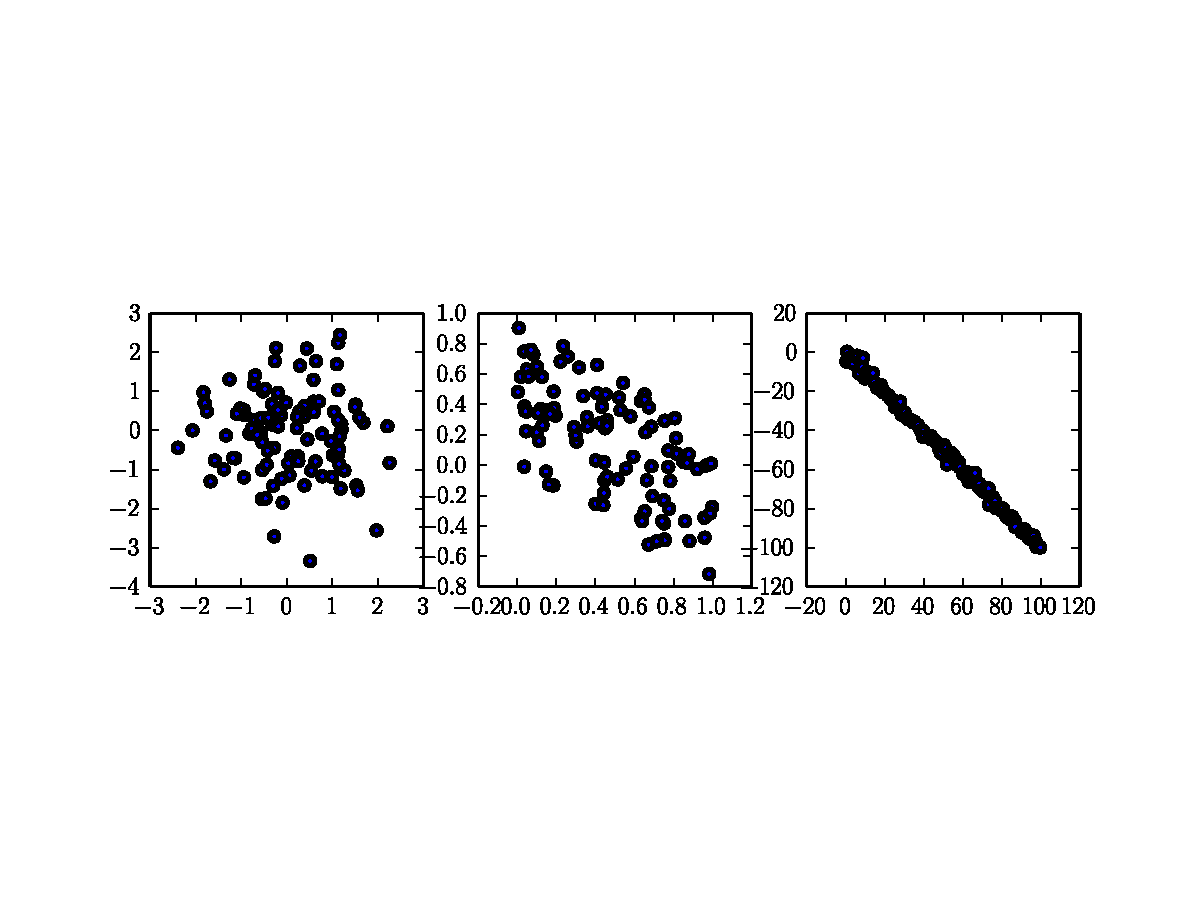
\includegraphics[width=\textwidth]{correlation}
\caption{Left: scatter plot of two slightly positively correlated vectors.
         Middle: scatter plot of two uncorrelated vectors.
         Right: scatter plot of two highly negatively correlated vectors.}
\label{fig:correlation}
\end{figure}

\begin{problem}
Import the data contained in the \li{mortality.txt} file. The first 17 rows are headers, providing the names of the
17 columns, and do not contain data. The first column is simply an index column, and may also be omitted.
The following 16 columns provide various demographic and environmental data for 60 countries, with the
final column giving the mortality rate for that country.
Distinct data entries are separated by whitespace.

Write a function that prints the answers to the following three questions, and generates plots as
described below.
Between which pair of distinct columns is the highest correlation?
Which column (apart from the last column) has the most negative correlation coefficient with mortality rate?
Which column is most nearly uncorrelated with mortality rate (i.e. the correlation coefficient is closest to 0)?
Make scatter plots of all three of these pairs of columns, and include them on the same subplot panel.
In all relevant cases, the mortality rate column should be the second argument passed to \li{plt.scatter}.
\end{problem}

It's important to understand that the high correlation between quantities does not necessarily imply
a causal relationship. For example, high correlation between violent crime rates and ice cream sales has
been observed. This does not mean that ice cream causes crime or that increases in crime makes people want
to eat more ice cream. Rather, both rates happen to increase during the summer and decrease during the winter.

Another import consideration is that the correlation coefficient does not provide information about
non-linear relationships and dependencies between data (see Figure \ref{fig:non_linear}). Any thorough analysis will go well beyond a simple
calculation of the correlation matrix.

\begin{figure}
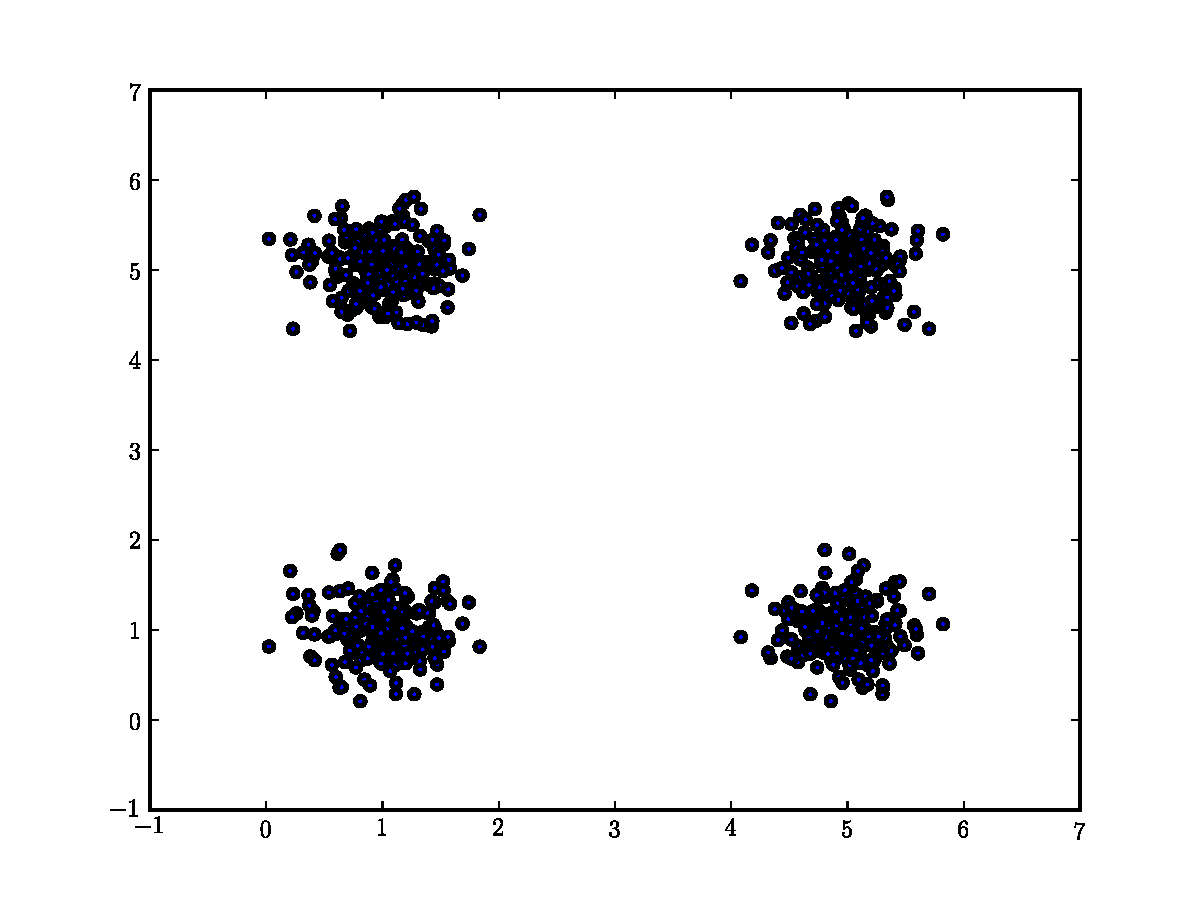
\includegraphics[width=\textwidth]{nonlinear_dependence}
\caption{There is a clear nonlinear relationship present in this data, but the Pearson correlation
         coefficient, which has a value of -0.00056, fails to capture it.}
\label{fig:non_linear}
\end{figure}

\section*{Covariance}
Related to the notion of correlation is that of covariance. 
The covariance of two vectors measures how they jointly vary together. 
In mathematical terms, given two vectors $u$ and $v$ in $\mathbb{R}^n$, with $\bar{u}$ and $\bar{v}$ denoting the mean-shifted 
versions of these vectors (as before), we define the \emph{covariance} of $u$ and $v$ to be
\[
\text{cov}(u,v) = \frac{\ipt{\bar{u}}{\bar{v}}}{n-1}.
\]
If $u$ and $v$ are close to parallel and both have high variance, then their covariance will be large in magnitude. 
On the other hand, if $u$ and $v$ are nearly orthogonal (that is, nearly uncorrelated), or one has very small variance,
then their covariance will be small in magnitude. 

Just as with correlation, we can generate a covariance matrix for a collection of vectors that contains the covariance for each set of vectors.
Specifically, given a collection of vectors $x_1,\ldots, x_m$, we define the covariance matrix $C$ for this collection to be the $m \times m$ matrix satisfying
\[
C_{i,j} = \text{cov}(u,v).
\]
If we let $X$ be the matrix whose columns are the mean-shifted vectors $\bar{x_1}, \ldots, \bar{x_m}$, note that
\begin{equation}
C = \frac{1}{n-1}X^TX.
\label{eq:cov}
\end{equation}
This gives us a very straight-forward way to compute the covariance matrix in Python:
\begin{lstlisting}
>>> # we will calculate the covariance matrix of W
>>> # subtract out the mean from the columns
>>> X = W-W.mean(axis=0)
>>> C = X.T.dot(X)/(X.shape[0]-1)
array([[ 303.33333333,  255.83333333,  222.33333333,  219.5       ],
       [ 255.83333333,  225.66666667,  196.        ,  184.5       ],
       [ 222.33333333,  196.        ,  205.66666667,  176.66666667],
       [ 219.5       ,  184.5       ,  176.66666667,  176.33333333]])
\end{lstlisting}
As usual, there is a nice way to compute the covariance matrix in NumPy, using the function \li{np.cov}. This function
also has the keyword argument \li{rowvar} which determines whether the covariance of the rows or of the columns is computed.
\begin{lstlisting}
>>> np.cov(W, rowvar=0)
array([[ 303.33333333,  255.83333333,  222.33333333,  219.5       ],
       [ 255.83333333,  225.66666667,  196.        ,  184.5       ],
       [ 222.33333333,  196.        ,  205.66666667,  176.66666667],
       [ 219.5       ,  184.5       ,  176.66666667,  176.33333333]])
\end{lstlisting}

\begin{problem}
Compute and report the covariance matrix of the \li{mortality.txt} data set. 
\end{problem}

Note that the covariance matrix is symmetric. 
Indeed, from equation \ref{eq:cov}, we can see that it is positive semi-definite and has nice spectral properties.
Observe from that same equation that the spectral decomposition of the covariance matrix is closely related to the singular value decomposition of $X$.
It turns out that the covariance matrix and its spectral properties contain much information about relationships, patterns, and structure in the data. 
Several statistical techniques in data compression, dimensionality reduction, and information retrieval rely on discovering and exploiting this structure,
and hence the covariance matrix and the singular value decomposition play an important role in data analysis. 

\section*{Latent Semantic Indexing}
We now have the tools to build a simple, yet effective, system for indexing and retrieving documents according to their semantic content.
The method that we will implement is called \emph{Latent Semantic Indexing}, or LSI.

Suppose we have a collection of documents, which we call a \emph{corpus}, and we wish to find the particular documents
that are most closely related to a given sequence of search terms. 
This problem arises when searching a database of newspaper articles, an email inbox, a scientific journal, and in many more settings. 
When our corpus consists of many documents, it becomes infeasible to read, or even skim, each document on our own. 
We need to utilize our mathematical and computational skills to facilitate the process.
To begin, we create a numerical representation of our corpus. 
A common approach, known as the \emph{vector space model}, is as follows. 
First, specify a list $v$ of words of interest (this could just be all the unique words found in the corpus).
Let $m$ be the length of the list $v$. Then we can represent a given document by a $m$-dimensional vector 
\[
d = \begin{bmatrix}
d_1 & d_2 & \cdots & d_m
\end{bmatrix}^T,
\]
where $d_i \in \mathbb{R}$ gives the contribution of the $i$-th term in the list $v$ to the document. 
For our purposes in this lab, we define $d_i$ to be the number of times term $i$ occurs in the document.
The following code snippet shows how to compute the vector representation of a document given a list of words.
We use a particular data structure \li{Counter}, which counts the number of occurrences of each unique element in a list.
\begin{lstlisting}
>>> from collections import Counter
>>> # initialize the word list and the document
>>> v = ["the", "great", "live", "math", "things", "do", "me", "you"]
>>> doc = "If you cannot do great things do small things in a great way"
>>> # split the document into a list of words, make counter
>>> count = Counter(doc.split())
>>> # create the vector representation
>>> d = np.array([count[w] for w in v])
>>> print d
[0 2 0 0 2 2 0 1]
\end{lstlisting}
If our corpus consists of $n$ documents, then we can represent the entire corpus by a $m \times n$ matrix
$D$ whose columns are just the vector representations of the documents. 
In most real-world applications, $m$ and $n$ are very large (in the several thousands, or more). 
Thankfully, the matrix $D$ will often be very sparse, since each particular document contains only a small subset
of the entire list of words.
Thus, we can use the sparse libraries in SciPy to efficiently store and compute with this matrix.

We now use the singular value decomposition to reduce the dimensionality of the matrix representation of our
corpus in a way that optimally decouples the semantic content of the documents. 
More precisely, we specify the number $t$ of greatest singular values we wish to retain, and calculate the truncated SVD of the matrix $D$,
yielding a rank-$t$ approximation
\[
D_t = U_t\Sigma_tV_t^T,
\]
where $U_t$ and $V_t$ are orthogonal matrices of size $m \times t$ and $n \times t$, respectively, and $\Sigma_t$
is a $t \times t$ diagonal matrix containing the $t$ largest singular values of $D$. 
A typical value for $t$ is in the low hundreds.
We can compute this in Python as follows:
\begin{lstlisting}
>>> from scipy.sparse import linalg as la
>>> # assume D is a sparse matrix
>>> t = 100
>>> U, Sig, VT = la.svds(D, k=t)
\end{lstlisting}
Although $U_t$ and $V_t$ are not sparse, they are much more feasible to compute with given that $t \ll m$. 
Observe that the $i$-th column of $V_t^T$ is $\Sigma_t^{-1}U_t^Td_i$, a transformed version of the $i$-th document vector.
It turns out that the matrix $\Sigma_t^{-1}U_t^T$ defines a projection from $\mathbb{R}^m$ onto a $t$-dimensional subspace
in such a way that the projections of semantically similar documents have high correlation in the subspace, and
semantically differing documents will have low correlation. 
Thus, if $q$ is the vector representation of a query, we can find the document in the corpus with the closest semantical
content to $q$ by projecting $q$ down to the $t$-dimensional subspace, calculating its correlation with each of the 
projected document vectors in the corpus, and then selecting the document with the highest such correlation.
\begin{comment}
The discussion above is still lacking, and doesn't quite hit the nail on the head. 
But I don't want it to become to wordy and bloated, so I'll leave it as is for now.
\end{comment}
\begin{lstlisting}
>>> # assume that docs is a list of the original documents
>>> # assume that q is the vector representation of a query
>>> # first, project q to the subspace
>>> q = (1/S)*(U.T.dot(q))
>>> # now calculate correlation of q with each column of VT
>>> q -= q.mean()           # shift by mean
>>> VT -= VT.mean(axis=0)
>>> q /= norm(q)            # normalize
>>> VT /= norm(VT, axis=0)
>>> coefs = VT.T.dot(q)
>>> # select the index of the highest correlation
>>> ind = np.argmax(coefs)
>>> print docs[ind]
\end{lstlisting}
\begin{problem}
Do LSI and stuff.
\end{problem}

As a final note, the concepts of variance, standard deviation, correlation, and covariance apply to a much broader class of objects
known as \emph{random variables}, which are central to statistics and probability theory. These topics will be
covered in detail later on.
